\documentclass[a4paper,12pt]{article}

% Packages
\usepackage[utf8]{inputenc}
\usepackage{geometry}
\usepackage{titlesec}
\usepackage{graphicx}
\usepackage{caption}
\usepackage{subcaption}
\usepackage{listings}
\usepackage{amsmath}
\usepackage{amssymb}                                                                                                                                                            
\usepackage{xcolor}

% Page setup
\geometry{a4paper, margin=1in}
\setlength{\parindent}{0pt}
\setlength{\parskip}{5pt}

% Title setup
\title{\textbf{DSP LAB - Experiment 7} \\
        \vspace*{0.3em}
        \large{Audio signal processing using HPF} \\}                                              
\author{Ajay Krishnan K \\  EE22BTECH11003}
\date{\today}

% Section and subsection formatting
\titleformat{\section}[block]{\normalfont\Large\bfseries}{\thesection}{1em}{}
\titleformat{\subsection}[block]{\normalfont\large\bfseries}{\thesubsection}{1em}{}
\titleformat{\subsubsection}[block]{\normalfont\normalsize\bfseries}{\thesubsubsection}{1em}{}

% Code listing settings
\lstdefinestyle{mystyle}{
    language=Matlab,
    basicstyle=\ttfamily\small,
    breaklines=true,
    keywordstyle=\color{blue},
    commentstyle=\color{green!40!black},
    stringstyle=\color{red},
    % numbers=left,
    % numberstyle=\tiny,
    frame=single,
    showspaces=false,
    showstringspaces=false,
}

\lstset{style=mystyle}

\begin{document}
\maketitle

\section*{Aim}
To investigate the effects of applying both low-pass and high-pass
filters on audio signals. Through this experiment, the aim is to
explore how these filters alter the frequency content
and perception of sound in order to gain insights into their
practical applications in audio processing and signal manipulation.

\section*{Theory}
\subsection*{Low Pass Filter}
A low-pass filter is a filter that passes signals with a frequency lower than a selected cutoff frequency and attenuates signals with frequencies higher than the cutoff frequency. The exact frequency response of the filter depends on the filter design.

\subsection*{High Pass Filter}
A high-pass filter is a filter that passes signals with a frequency higher than a certain cutoff frequency and attenuates signals with frequencies lower than the cutoff frequency. The exact frequency response of the filter depends on the filter design.

\section*{Design}
The LPF and HPF are designed using the following specifications:
\begin{itemize}
    \item LPF: Cutoff frequency = 10 kHz
    \item HPF: Cutoff frequency = 10 kHz
\end{itemize}

\section*{MATLAB Code}
The function \texttt{LPF} for the low-pass filter is given below: 
\lstinputlisting[language=Matlab]{../code/LPF.m}

The function \texttt{HPF} for the high-pass filter is given below:
\lstinputlisting[language=Matlab]{../code/HPF.m}

The script to generate the plots is given below:
\lstinputlisting[language=Matlab]{../code/lab7.m}

\section*{Outputs}

The specgram plot of the original input wave is given in Figure \ref{fig:specgramOg}.
\begin{figure}[h]
    \centering
    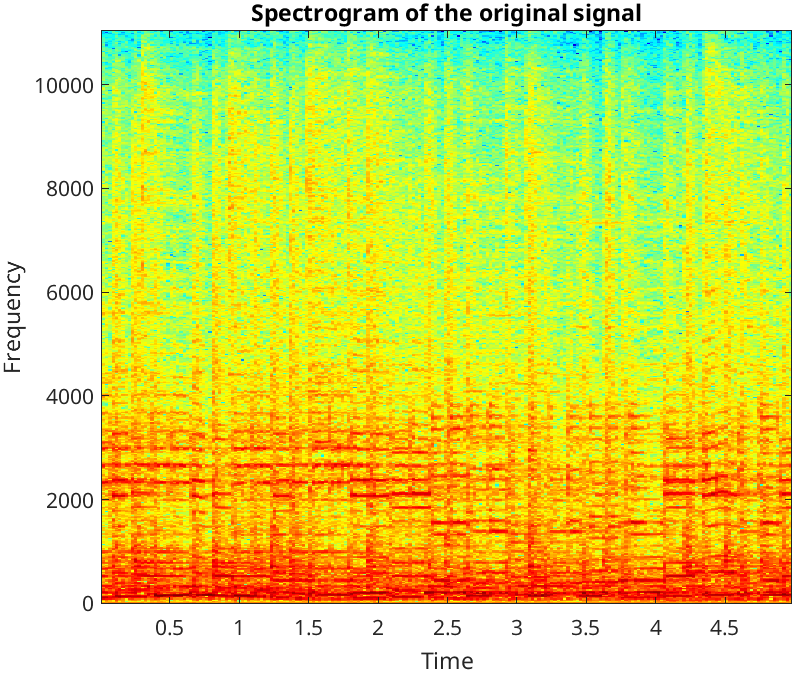
\includegraphics[width=0.8\textwidth]{figs/specOg.png}
    \caption{Specgram of the original wave}
    \label{fig:specgramOg}
\end{figure}

\subsection*{Low Pass Filter (LPF)}
The impulse response of the LPF is given in Figure \ref{fig:impulseLPF}.
\begin{figure}[h]
    \centering
    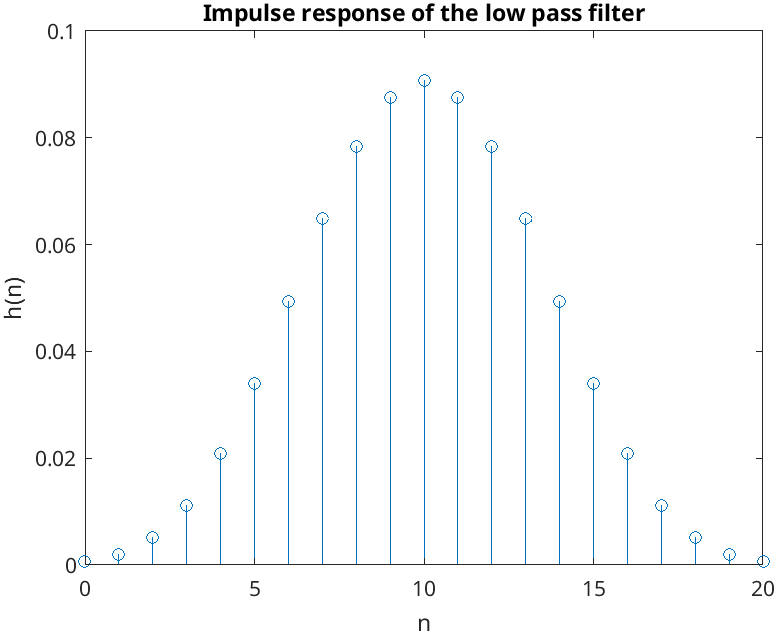
\includegraphics[width=0.8\textwidth]{figs/impulseLPF.png}
    \caption{Impulse response of the LPF}
    \label{fig:impulseLPF}
\end{figure}


The magnitude response of the LPF is given in Figure \ref{fig:magnitudeLPF}.
\begin{figure}[h]
    \centering
    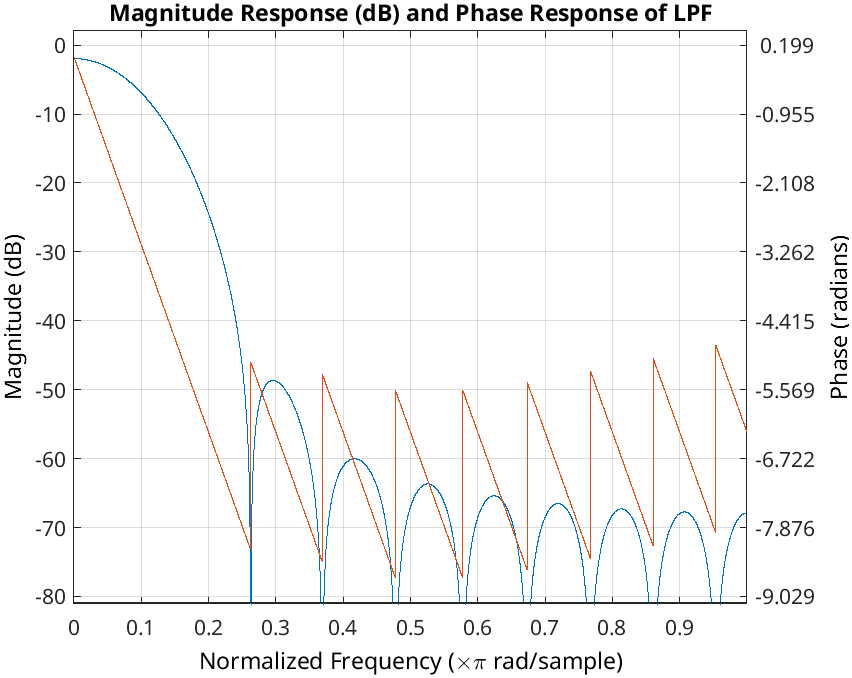
\includegraphics[width=0.8\textwidth]{figs/magLPF.png}
    \caption{Magnitude response of the LPF}
    \label{fig:magnitudeLPF}
\end{figure}

The specgram plot of the output wave after passing through the LPF is given in Figure \ref{fig:specgramLPF}.
\begin{figure}[h]
    \centering
    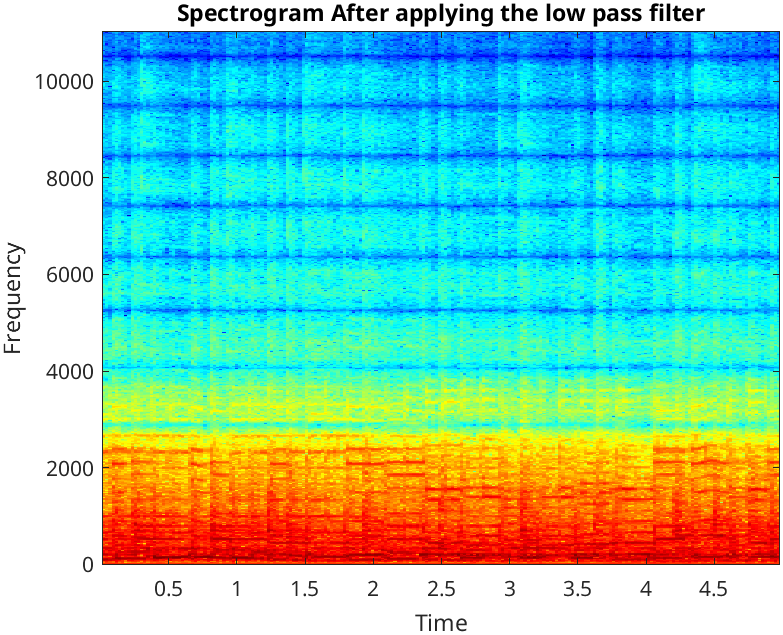
\includegraphics[width=0.8\textwidth]{figs/specLPF.png}
    \caption{Specgram of the LPF output}
    \label{fig:specgramLPF}
\end{figure}

\subsection*{High Pass Filter (HPF)}

The impulse response of the HPF is given in Figure \ref{fig:impulseHPF}.
\begin{figure}[h]
    \centering
    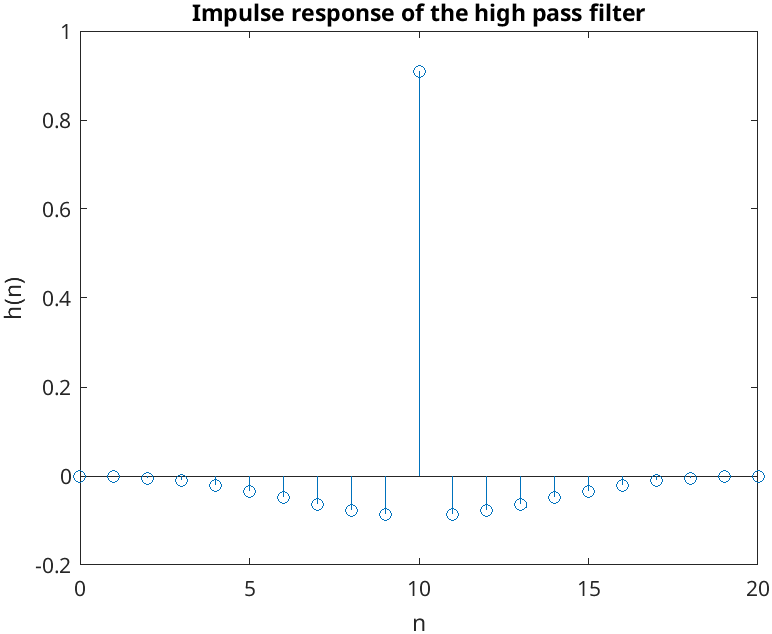
\includegraphics[width=0.8\textwidth]{figs/impulseHPF.png}
    \caption{Impulse response of the HPF}
    \label{fig:impulseHPF}
\end{figure}

The magnitude response of the HPF is given in Figure \ref{fig:magnitudeHPF}.
\begin{figure}[h]
    \centering
    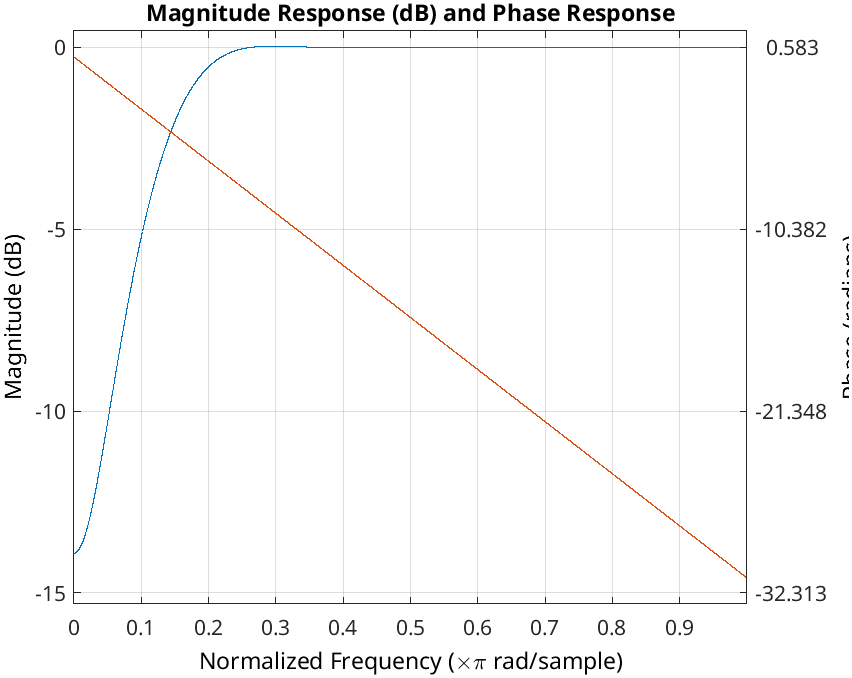
\includegraphics[width=0.8\textwidth]{figs/magHPF.png}
    \caption{Magnitude response of the HPF}
    \label{fig:magnitudeHPF}
\end{figure}

The specgram plot of the output wave after passing through the HPF is given in Figure \ref{fig:specgramHPF}.
\begin{figure}[!h]
    \centering
    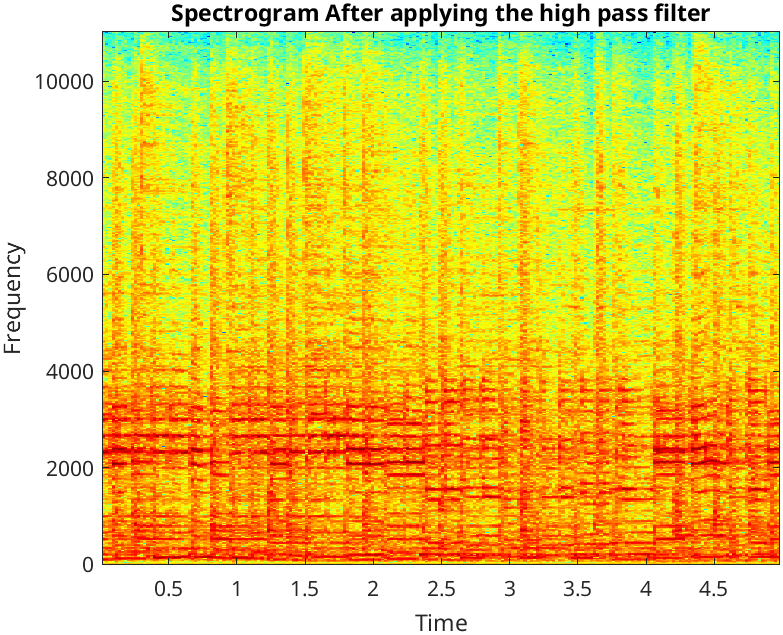
\includegraphics[width=0.8\textwidth]{figs/specHPF.png}
    \caption{Specgram of the HPF output}
    \label{fig:specgramHPF}
\end{figure}

\section*{Observations}
\begin{itemize}
    \item HPF can be obtained from an LPF by shifting the frequency response by $\pi$.
    \item The LPF attenuates the high frequency components of the audio signal, resulting in a smoother and less sharp sound.
    \item The HPF attenuates the low frequency components of the audio signal, resulting in a sharper and more pronounced sound.
    \item The LPF output has a more muffled and less distinct sound compared to the original signal, while the HPF output has a more crisp and clear sound.
    \item As the order of the filter increases, the sharpness of the filter increases and the specgram becomes more clear.
    \item The original wave has a lot of low frequency components, which are attenuated by the HPF, resulting in a more pronounced high frequency sound.
\end{itemize}

\section*{Conclusion}
The experiment demonstrates the effects of applying low-pass and high-pass filters on audio signals. The LPF attenuates high frequency components, resulting in a smoother sound, while the HPF attenuates low frequency components, resulting in a sharper sound. The LPF output is more muffled and less distinct compared to the original signal, while the HPF output is more crisp and clear. The experiment provides insights into the practical applications of LPF and HPF in audio processing and signal manipulation.
It also shows that HPF can be obtained from an LPF by shifting the frequency response by $\pi$.
\end{document}